\chapter{Thiết kế giao diện người diện}

\section{Trang chào mừng}

\begin{figure}[H]
\begin{center}
    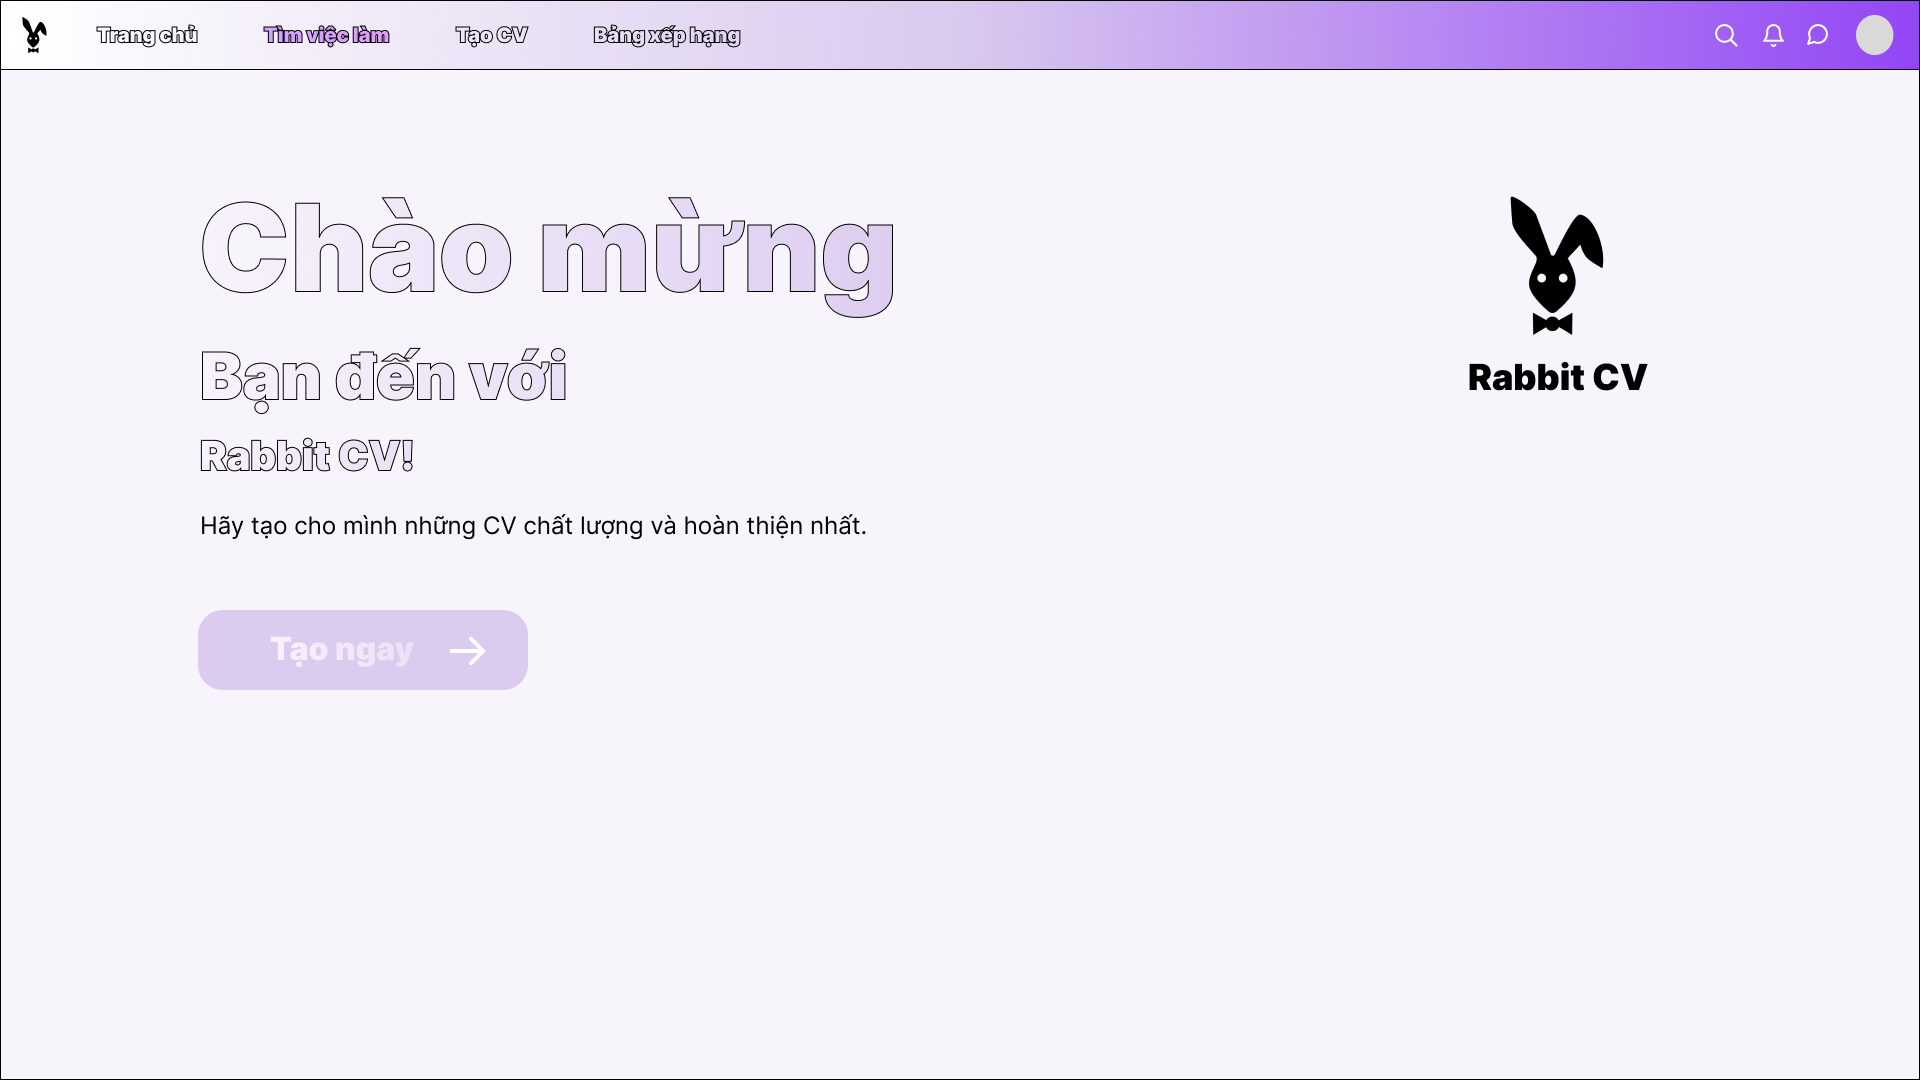
\includegraphics[scale=0.2]{img/Welcome.png}
    \caption{Giao diện của Trang chào mừng}
\end{center}
\end{figure}

Trang chào mừng của một trang web là điểm tiếp xúc đầu tiên giữa người dùng và nội dung của trang web đó. Đây là nơi mà người dùng sẽ có ấn tượng đầu tiên về trang web, và do đó, nó cần phải được thiết kế một cách cẩn thận và chuyên nghiệp.

Trang chào mừng của một trang web đóng vai trò quan trọng trong việc tạo ấn tượng đầu tiên với người dùng. Đây là nơi mà người dùng sẽ quyết định liệu họ có muốn tiếp tục khám phá trang web hay không. Một trang chào mừng hiệu quả không chỉ cần có thiết kế đẹp mắt mà còn phải cung cấp thông tin rõ ràng và dễ hiểu về nội dung và mục đích của trang web. 

Do đó, việc thiết kế giao diện của trang chào mừng cần phải thân thiện với người dùng và dễ dàng điều hướng.

\section{Trang đăng nhập}

\begin{figure}[H]
\begin{center}
    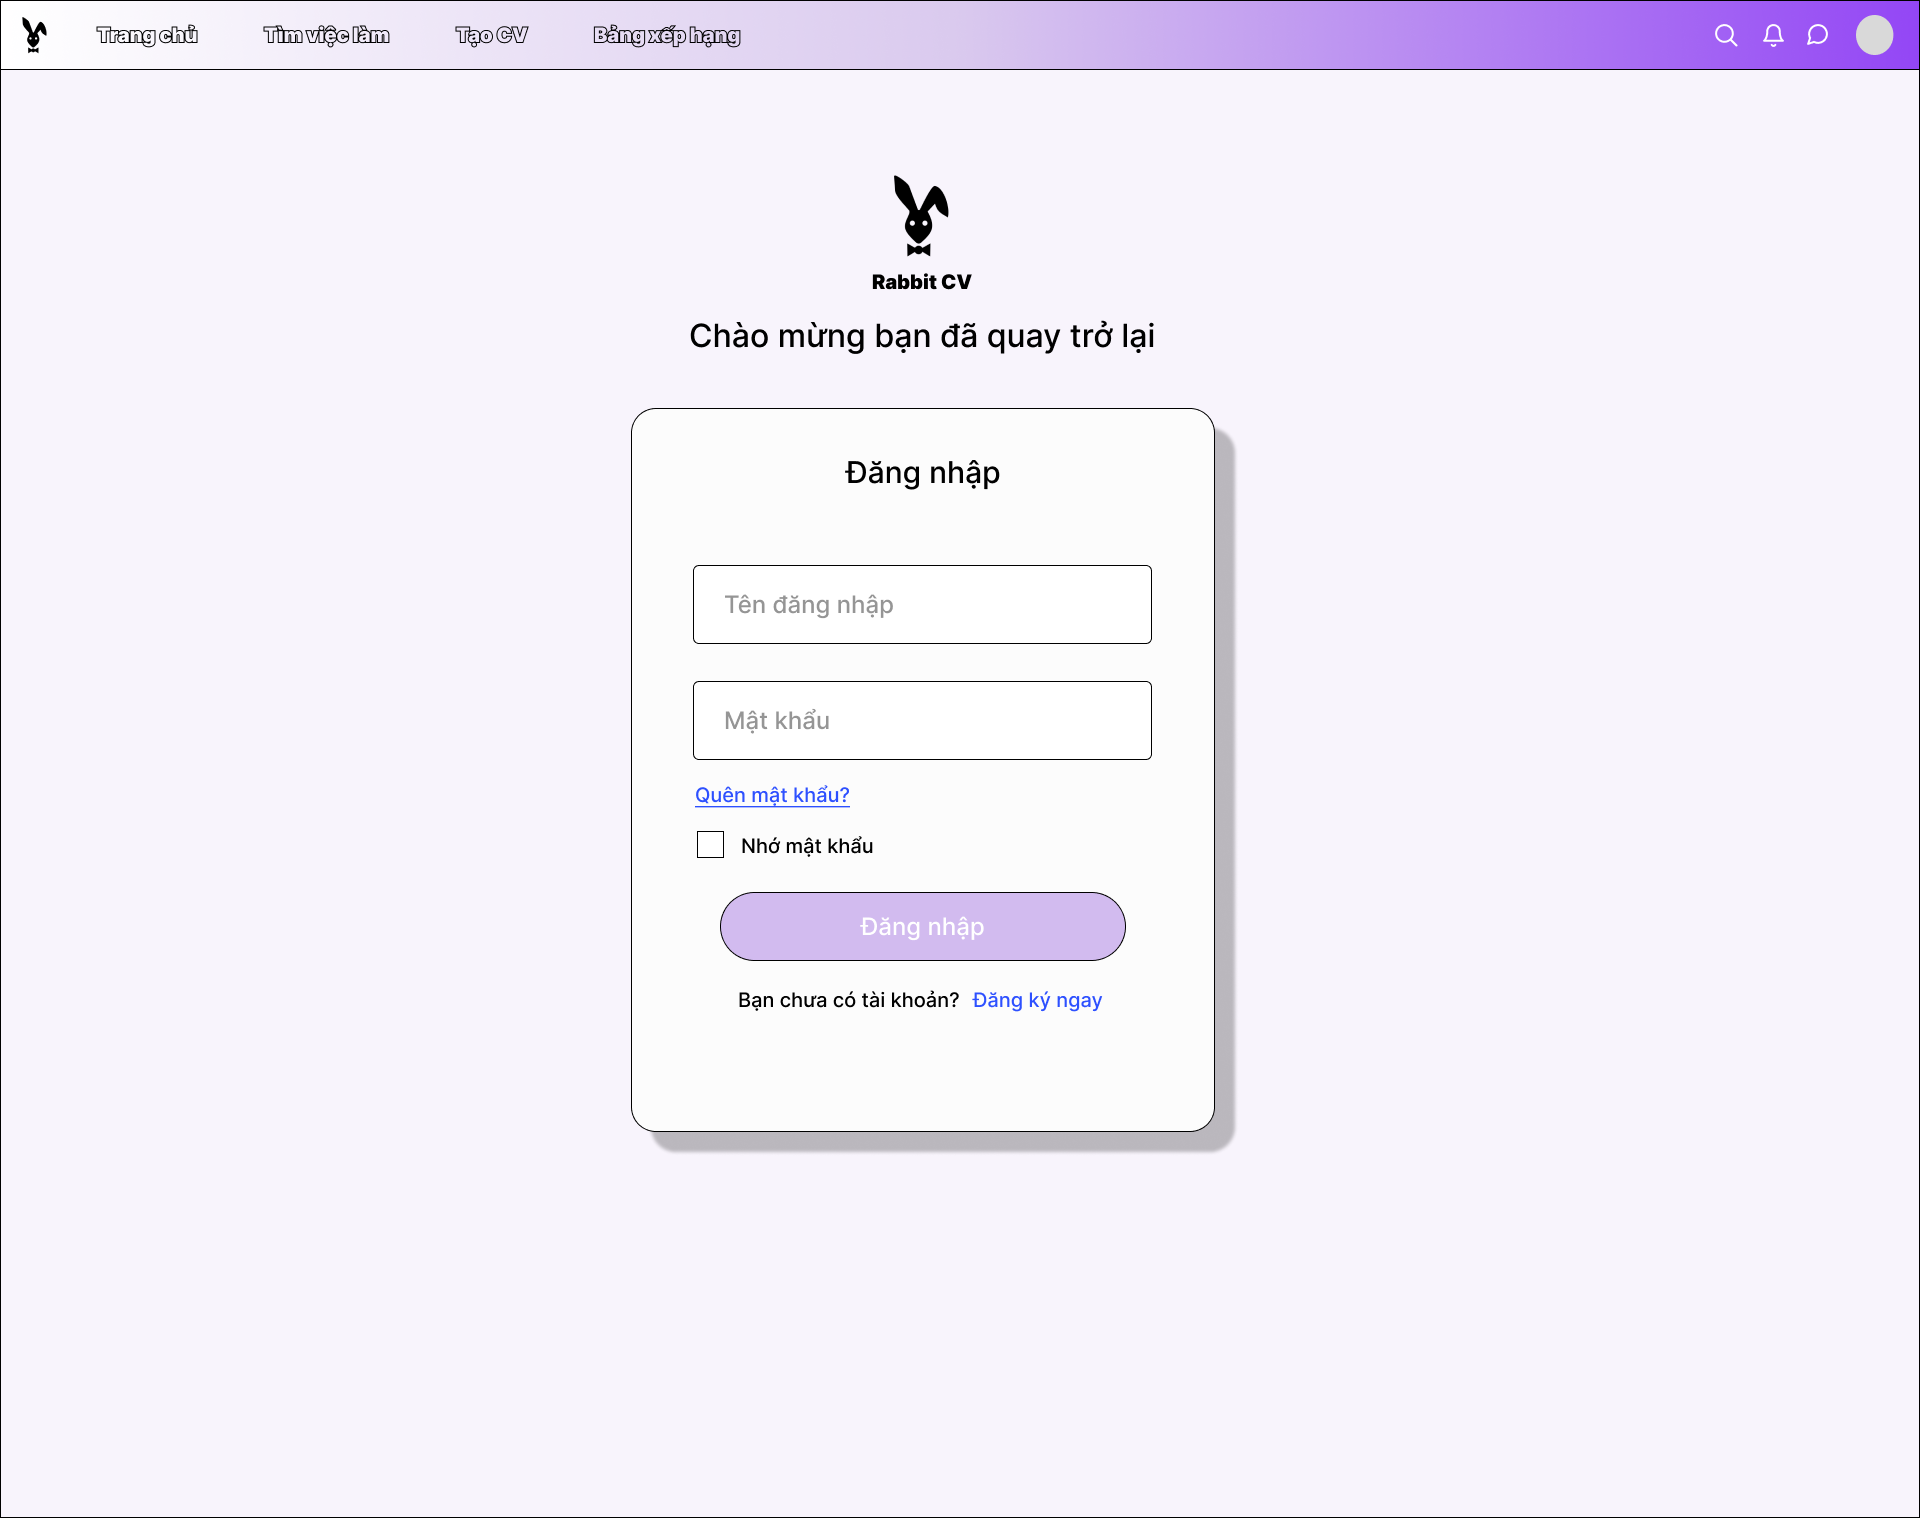
\includegraphics[scale=0.2]{img/Login.png}
    \caption{Giao diện của Trang đăng nhập}
\end{center}
\end{figure}

Trang đăng nhập là một phần quan trọng của bất kỳ trang web hoặc ứng dụng nào yêu cầu người dùng xác thực danh tính trước khi truy cập vào các tính năng hoặc dữ liệu cá nhân. Trang đăng nhập cũng có nhiều tuỳ chọn khác như: "Đăng ký tài khoản mới", "Quên tài khoản",.... 

Trang đăng nhập bao gồm các thành phần:

\begin{itemize}
    \item \textbf{Tên đăng nhập:} người dùng được yêu cầu phải điền vào trang web.
    \item \textbf{Mật khẩu:} Được yêu cầu điền để kiểm tra mật khẩu ứng với tên đăng nhập trong cơ sở dữ liệu.
    \item \textbf{Quên mật khẩu:} Là một đường link được chuyển hướng đến trang "Quên mật khẩu" khi người dùng thực sự quên mật khẩu, tài khoản của mình.
    \item \textbf{Nhớ mật khẩu:} Là một tuỳ chọn giúp người dùng có thể tự động đăng nhập ở các phiên đăng nhập sau.
    \item \textbf{Đăng nhập:} Là một nút để đăng nhập khi người dùng đã điền thông tin tài khoản và mật khẩu. Khi đăng nhập, hệ thông sẽ kiểm tra tài khoản và mật khẩu của người dùng có trong cơ sở dữ liệu của hệ thống hay không.
    \item \textbf{Đăng ký ngay:} Là đường link chuyển hướng tới trang "Đăng ký tài khoản". Nếu người dùng vẫn chưa có tài khoản trong cơ sở dữ liệu của hệ thống, người dùng có thể lựa chọn tuỳ chọn này để tạo tài khoản mới.
\end{itemize}

\section{Trang đăng ký}

\begin{figure}[H]
\begin{center}
    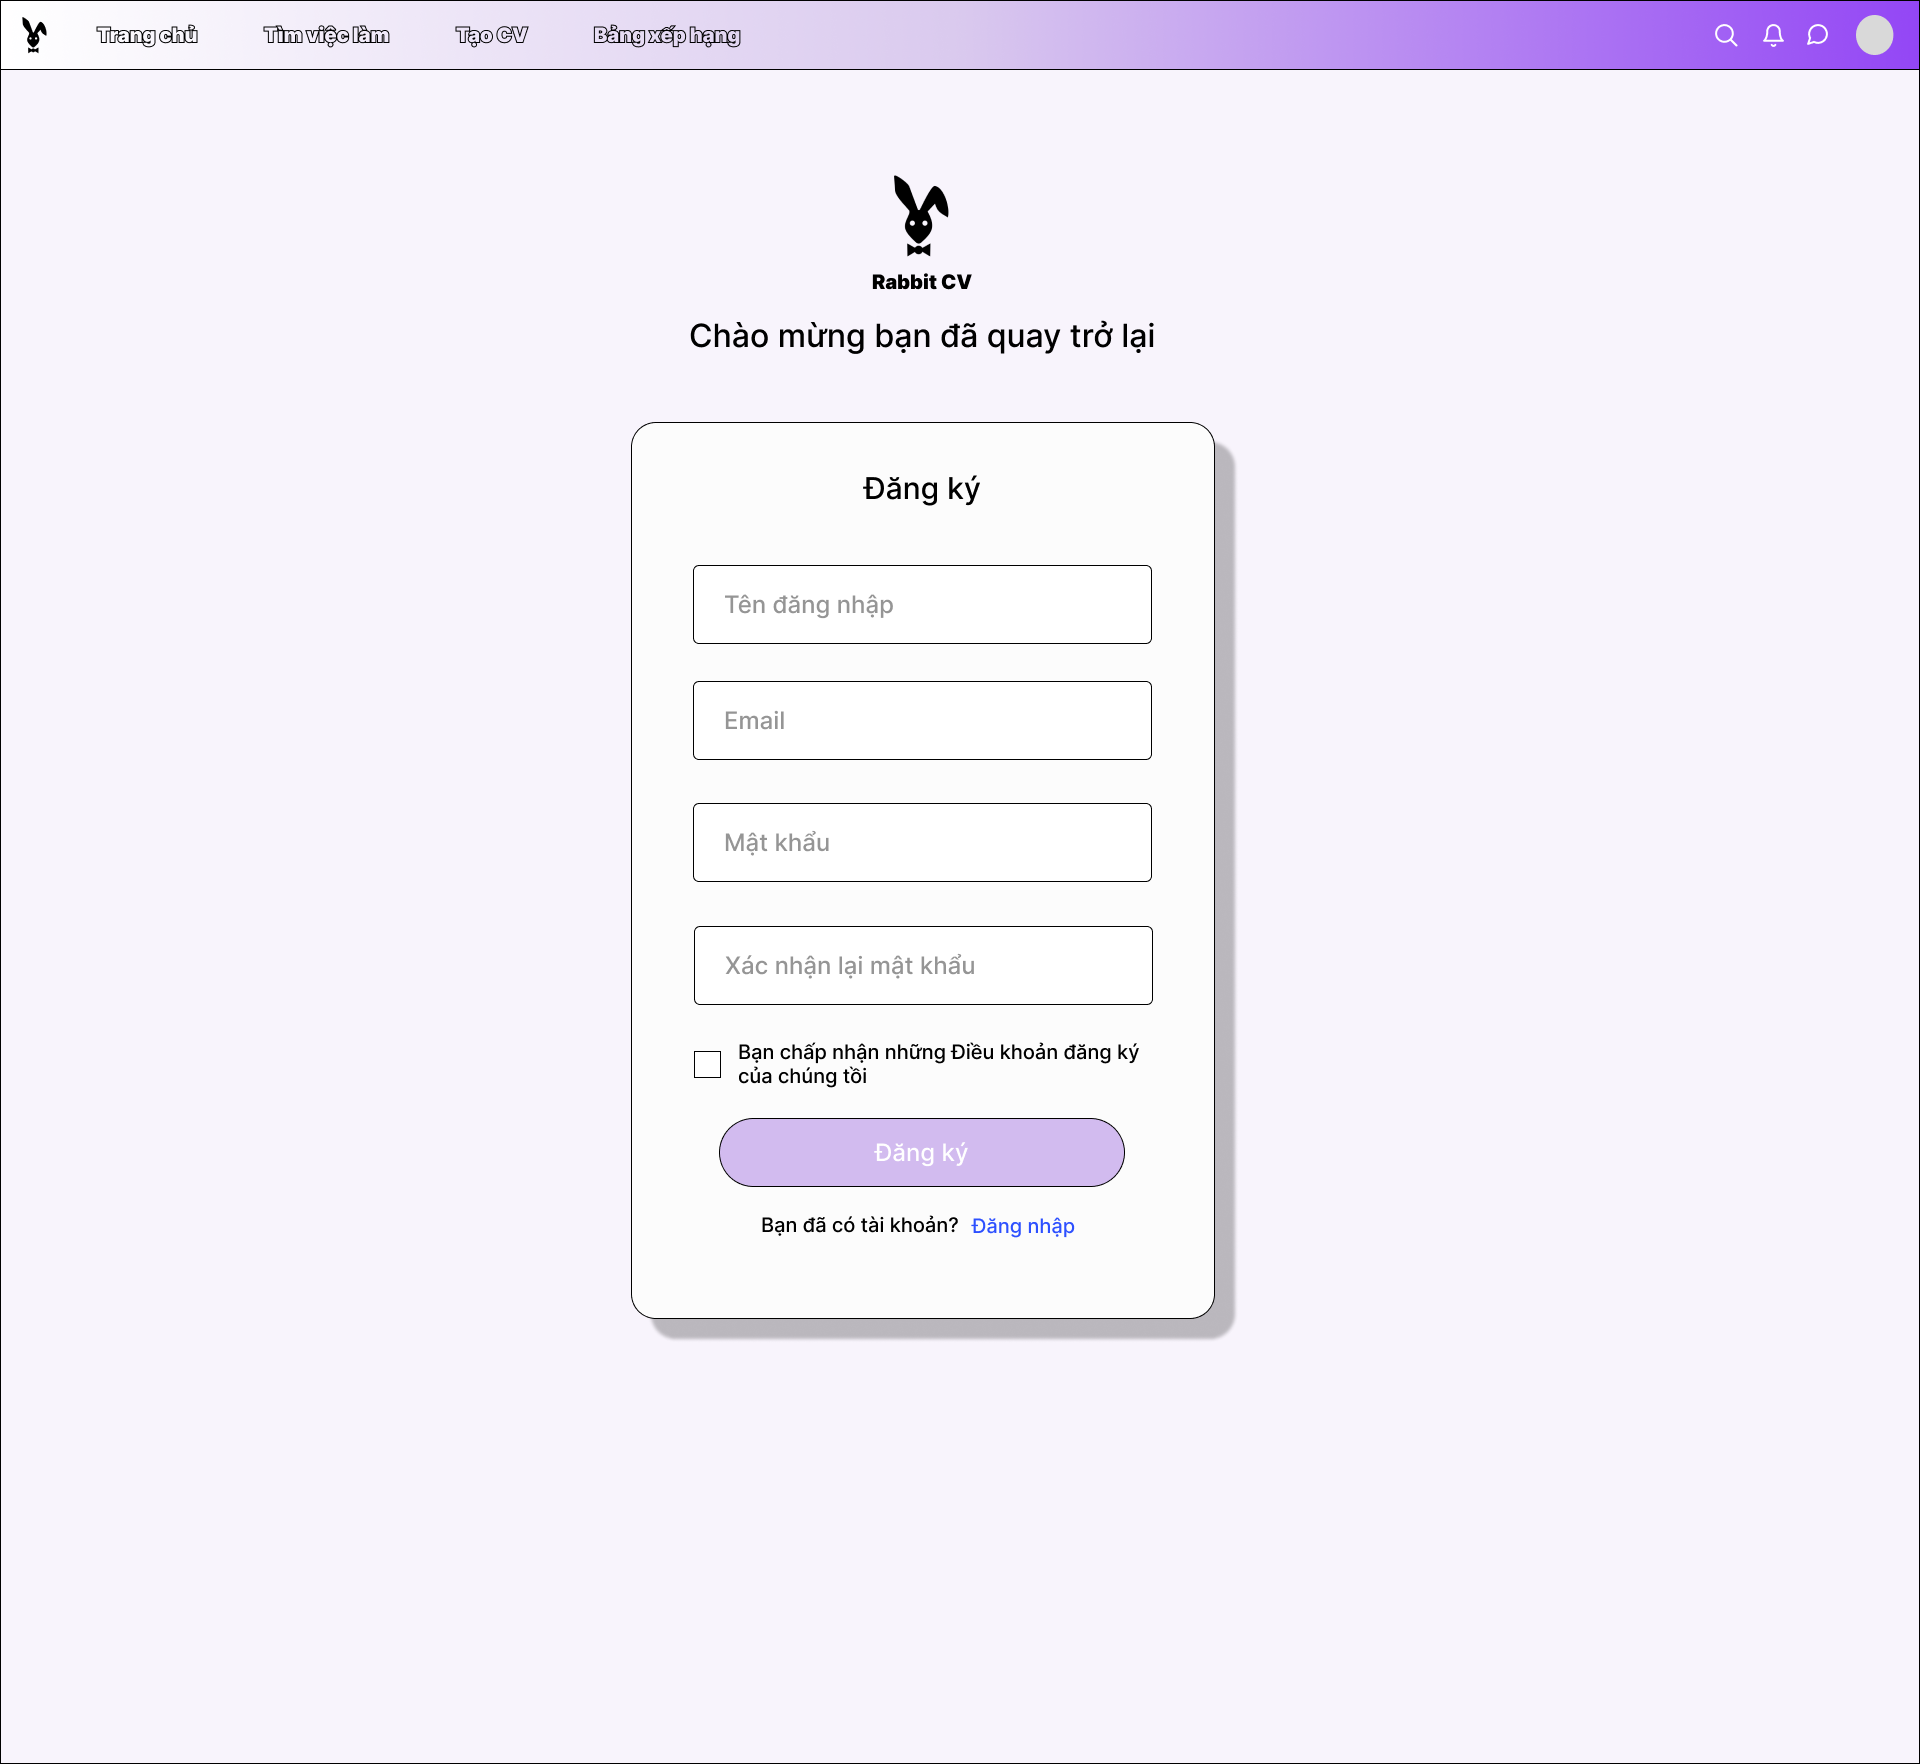
\includegraphics[scale=0.2]{img/Register.png}
    \caption{Giao diện Trang đăng ký}
\end{center}
\end{figure}

Là trang web yêu cầu người dùng tạo tài khoản mới để có truy cập vào các tính năng và dịch vụ của trang web. Để đăng ký tài khoản mới, người dùng cần phải đồng ý với các điều khoản, điều kiện đăng ký của trang web.

Trang đăng ký có các thành phần:
\begin{itemize}
    \item \textbf{Tên đăng nhập:} Là trường yêu cầu người dùng phải nhập tên đăng nhập của mình. 
    \item \textbf{Email:} Là trường người dùng được yêu cầu phải nhập để sau này khi người dùng quên mật khẩu, hệ thống có thể dựa vào đó để xác minh người dùng.
    \item \textbf{Mật khẩu:} Là trường để người dùng đặt mật khẩu. Ở trường này, mật khẩu sẽ được dấu dưới dạng ký hiệu *, để dấu mật khẩu trước những người khác ở trước màn hình. Người dùng cũng có thể lựa chọn nhìn mật khẩu nếu họ thực sự muốn.
    \item \textbf{Xác nhận mật khẩu:} Là trường để xác nhận lại với người dùng mật khẩu mà họ đã chọn .
    \item \textbf{Đăng ký:} Là nút khi người dùng nhấn vào, hệ thống sẽ kiểm tra lại cơ sở dữ liệu xem tài khoản mà người dùng chọn đã có người khác xài chưa. Nếu đã có, thì hệ thống sẽ thông báo "Tạo tài khoản thất bại" và yêu cầu người chọn một tên tài khoản khác. Còn nếu chưa, hệ thống sẽ thông báo "Tạo tài khoản thành công" và đưa người dùng đến trang đăng nhập.
    \item \textbf{Đăng nhập:} Là đường link chuyển hướng người dùng đến trang "Đăng nhập". Nếu người dùng đã có tài khoản trong cơ sở dữ liệu của hệ thống, họ có thể lựa chọn chức năng này.
\end{itemize}


\section{Trang chủ}

\begin{figure}[H]
\begin{center}
    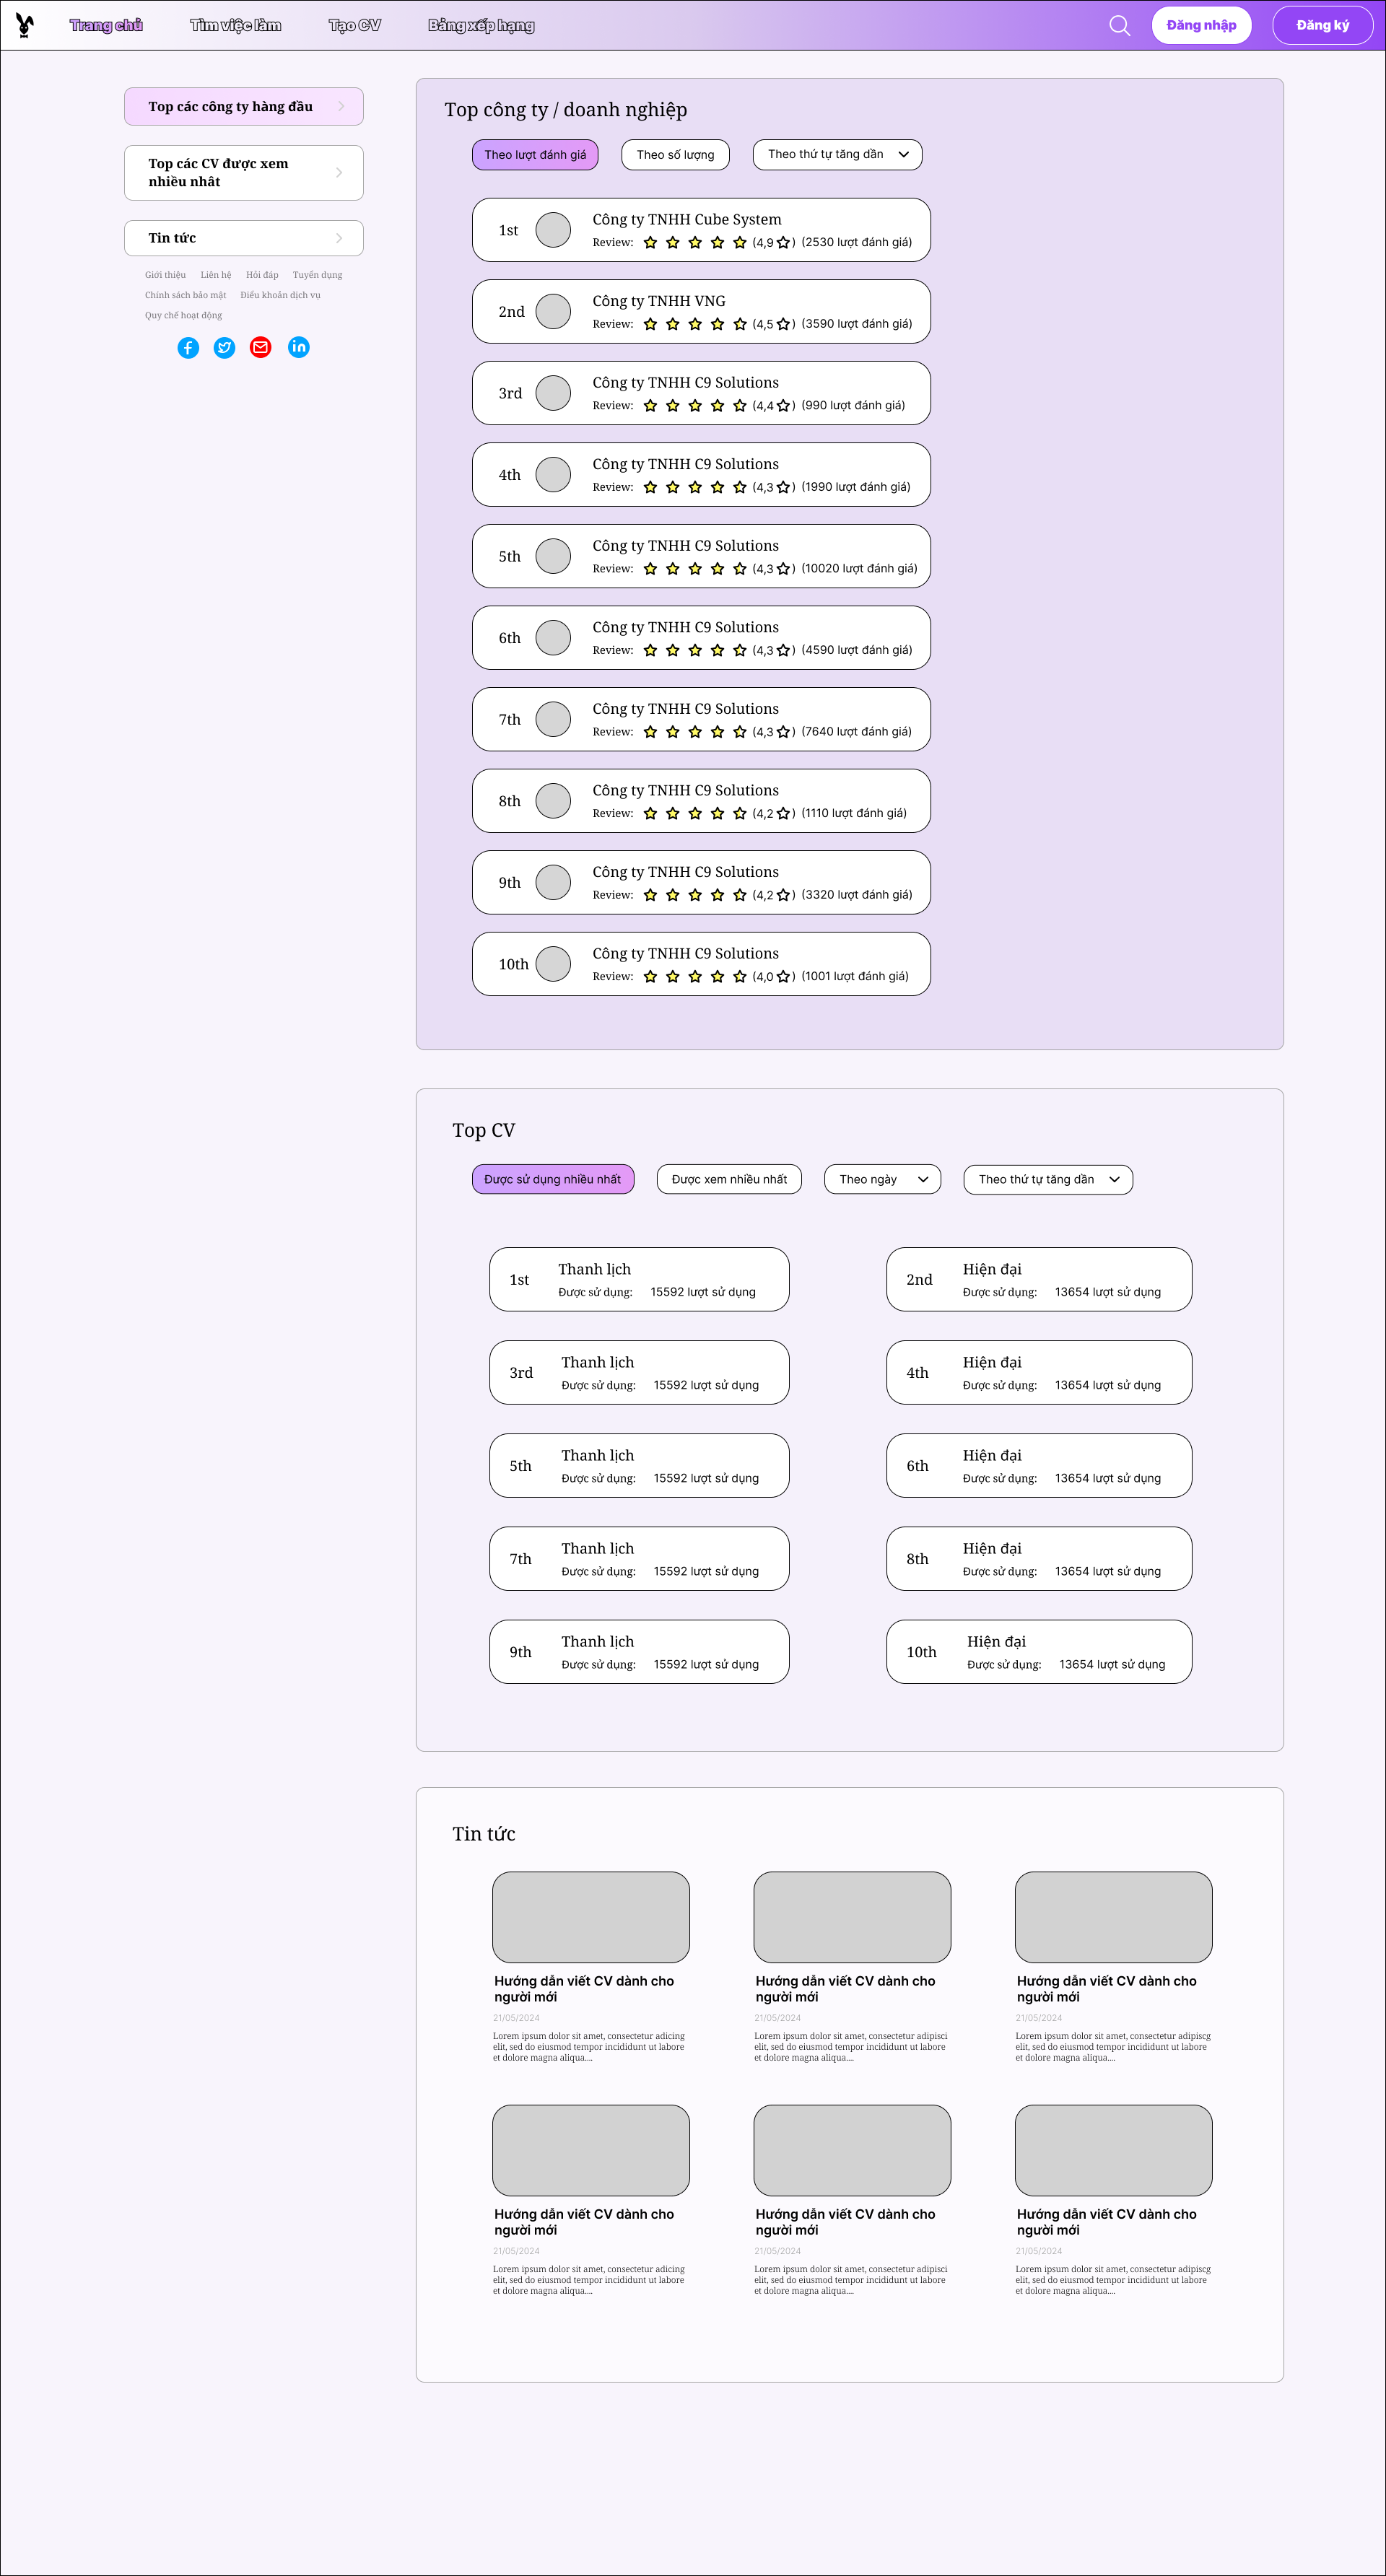
\includegraphics[scale=0.15]{img/Homepage.png}
    \caption{Giao diện của Trang chủ}
\end{center}
\end{figure}

Trang chủ của một trang web là điểm đầu tiên và quan trọng nhất mà người dùng sẽ truy cập. Đây là nơi cung cấp cái nhìn tổng quan về nội dung và dịch vụ mà trang web cung cấp. Trang web này cũng là cổng thông tin chính giúp người dùng dễ dàng điều hướng và tìm kiếm thông tin.

Ở trang web này, gồm có 3 mục: Top doanh nghiệp, Top CV và Tin tức. Ở mảng bên trái sẽ có một danh sách gồm các danh mục vừa được nêu giúp người dùng có thể chọn và nhanh chóng di chuyển đến mục đã được chọn.


\section{Trang tìm kiếm công việc}

\begin{figure}[H]
\begin{center}
    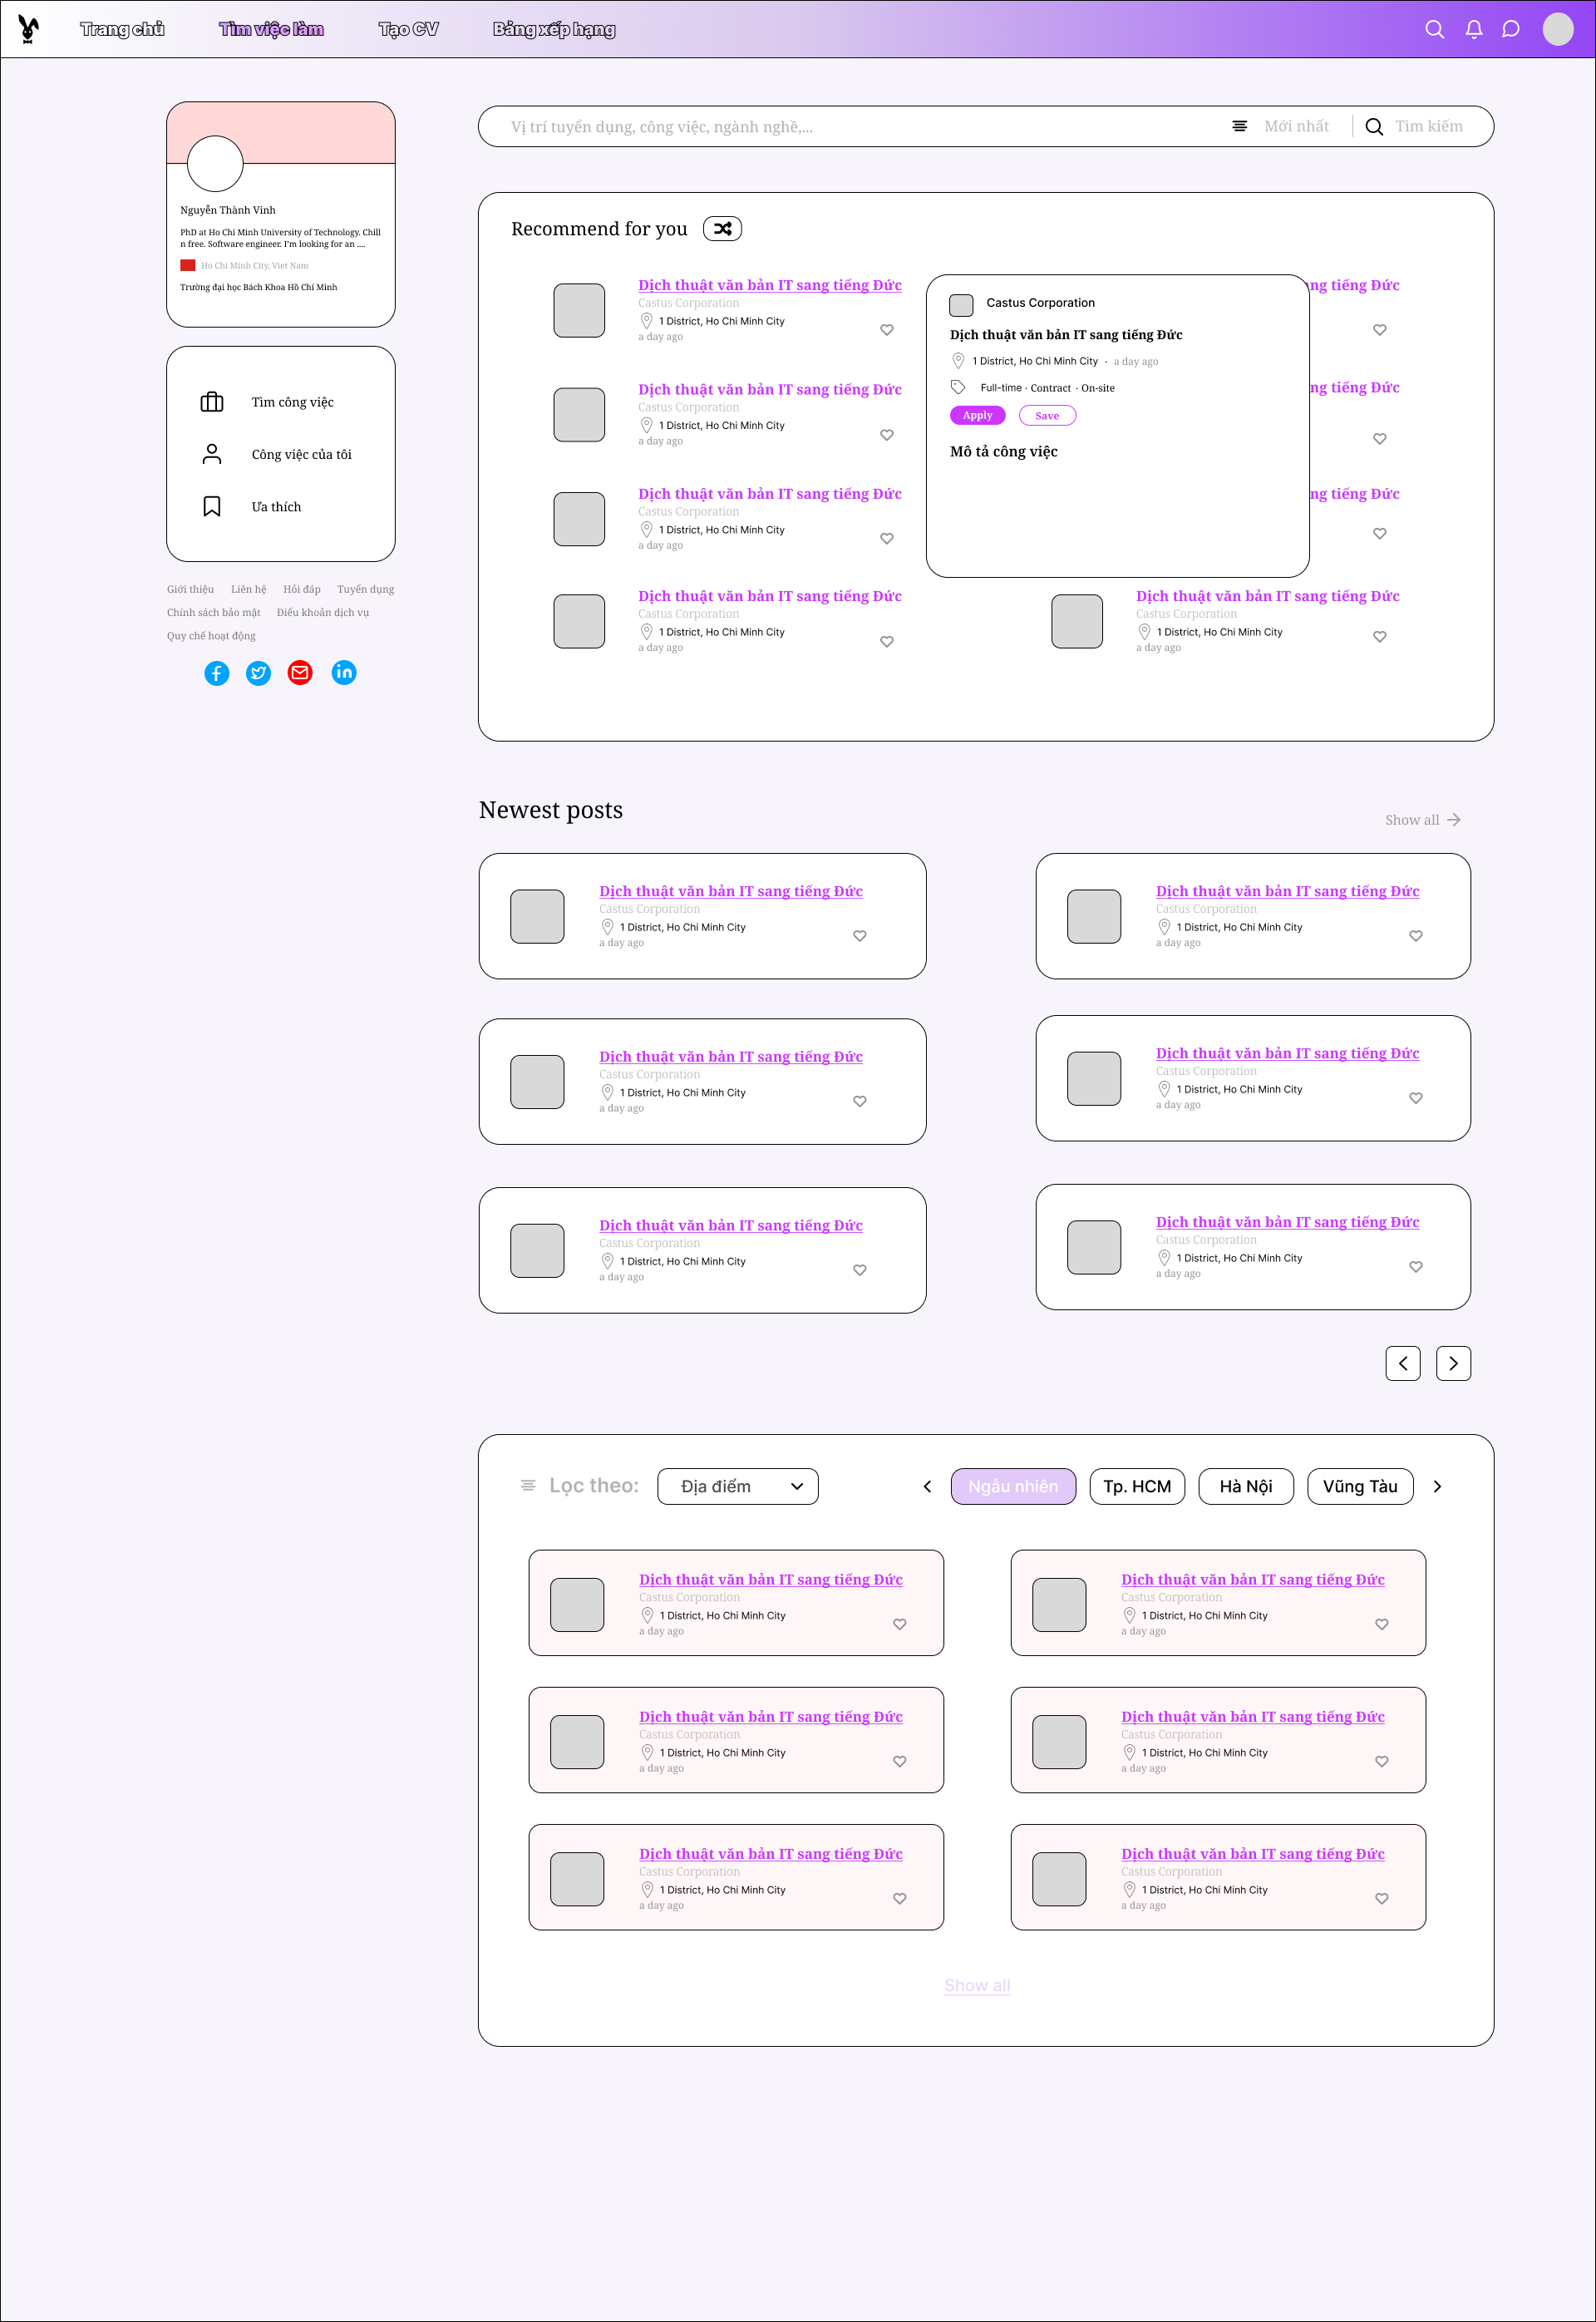
\includegraphics[scale=0.2]{img/FindingJob.png}
    \caption{Giao diện của Trang tìm kiếm công việc}
\end{center}
\end{figure}

Trang tìm kiếm công việc là trang hiển thị những bài đăng tuyển dụng của các doanh nghiệp. Ở đây, có 3 phần: "Recommend for you" gồm những bài đăng ngẫu nhiên được hệ thống đưa lên hệ thống, "Newest posts" gồm những bài đăng mới nhất, gần đây nhất và mục lọc danh sách những bài đăng tuỳ theo vị trí, lương, kinh nghiệm,.... 

\section{Trang quản lý CV}

\begin{figure}[H]
\begin{center}
    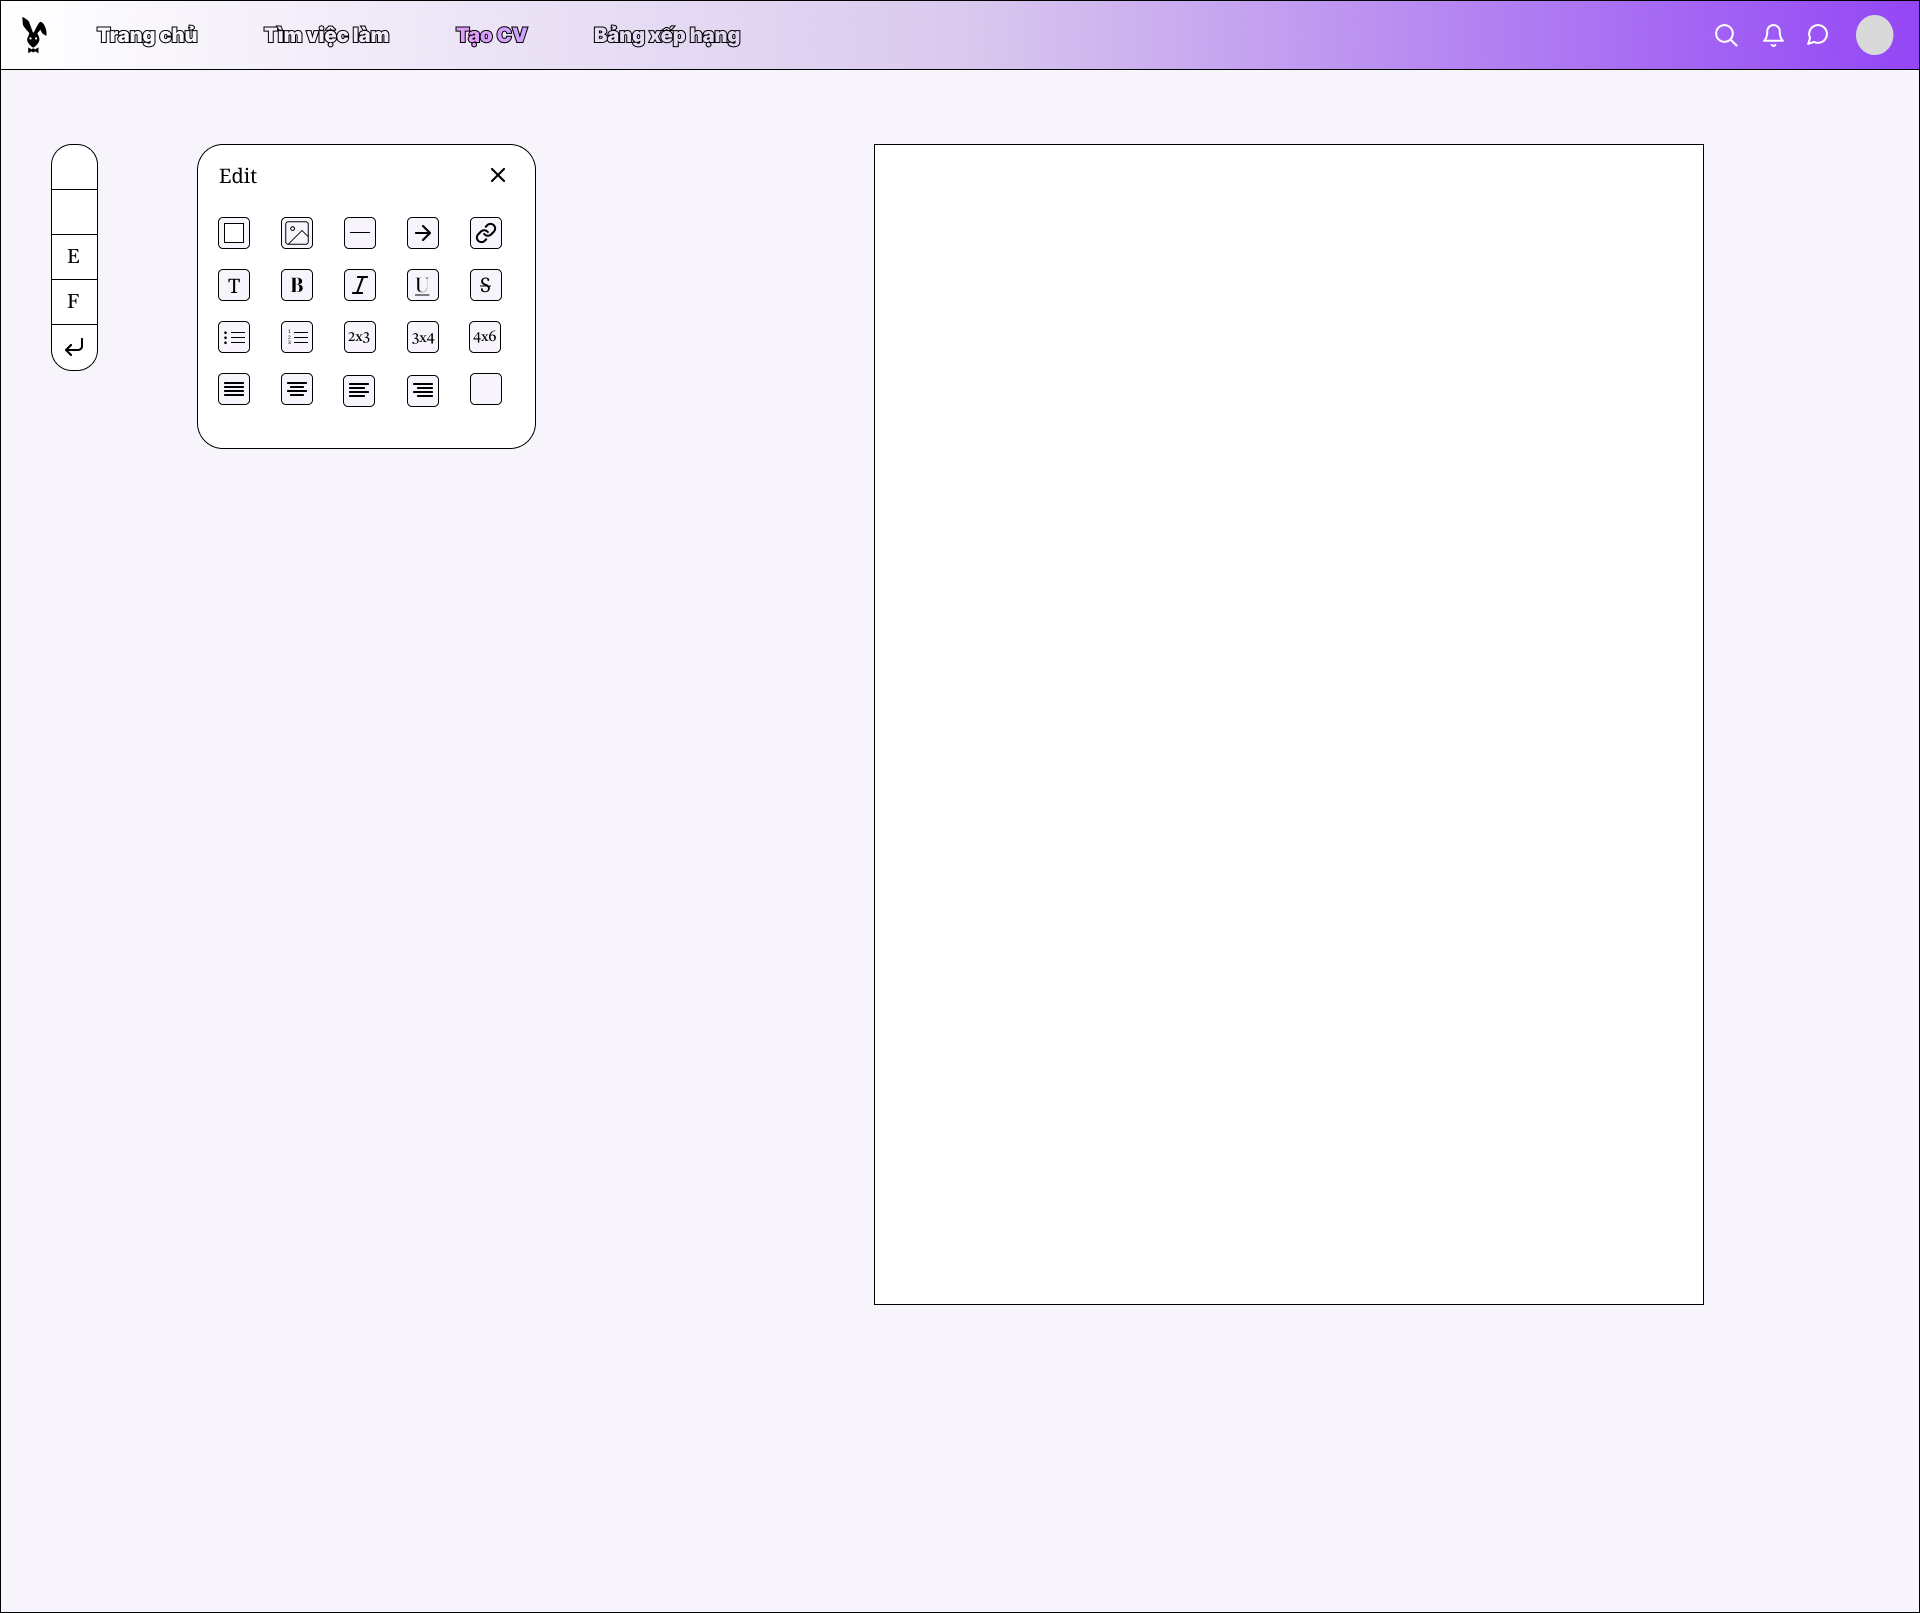
\includegraphics[scale=0.2]{img/CV_Management.png}
    \caption{Giao diện của Trang quản lý CV}
\end{center}
\end{figure}

Là trang để người dùng quản lý CV của mình. Trang này cung cấp cho người dùng các công cụ và tính năng để tạo, chỉnh sửa và xoá CV của họ một cách nhanh chóng và hiệu quả. Trang quản lý CV không chỉ giúp người dùng tạo ra những bản CV ấn tượng mà còn giúp người dùng dễ dàng quản lý và dễ dàng cập nhật thông tin, từ đó, nâng cao cơ hội tìm kiếm việc làm thành công.

Việc chỉnh sửa CV sẽ tuỳ thuộc vào tuỳ chọn mà người dùng đã chọn. Nếu dùng chọn CV template có trên trang web, hệ thống sẽ hiển thị sẵn một bản mẫu CV có sẵn và việc người dùng cần làm là chỉ điền thông tin cần thiết vào CV. Còn nếu người dùng chọn mục "Custom", hệ thống sẽ chỉ hiển thị 1 trang A4 lên trang web và những công cụ hữu ích hỗ trợ người dùng trong việc tự mình chỉnh sửa CV. Ở mục "Custom", người dùng có thể tự do chỉnh sửa, căn chỉnh hình ảnh, cỡ chữ phù hợp với yêu cầu của mình.



\section{Trang quản lý tài khoản}

\begin{figure}[H]
\begin{center}
    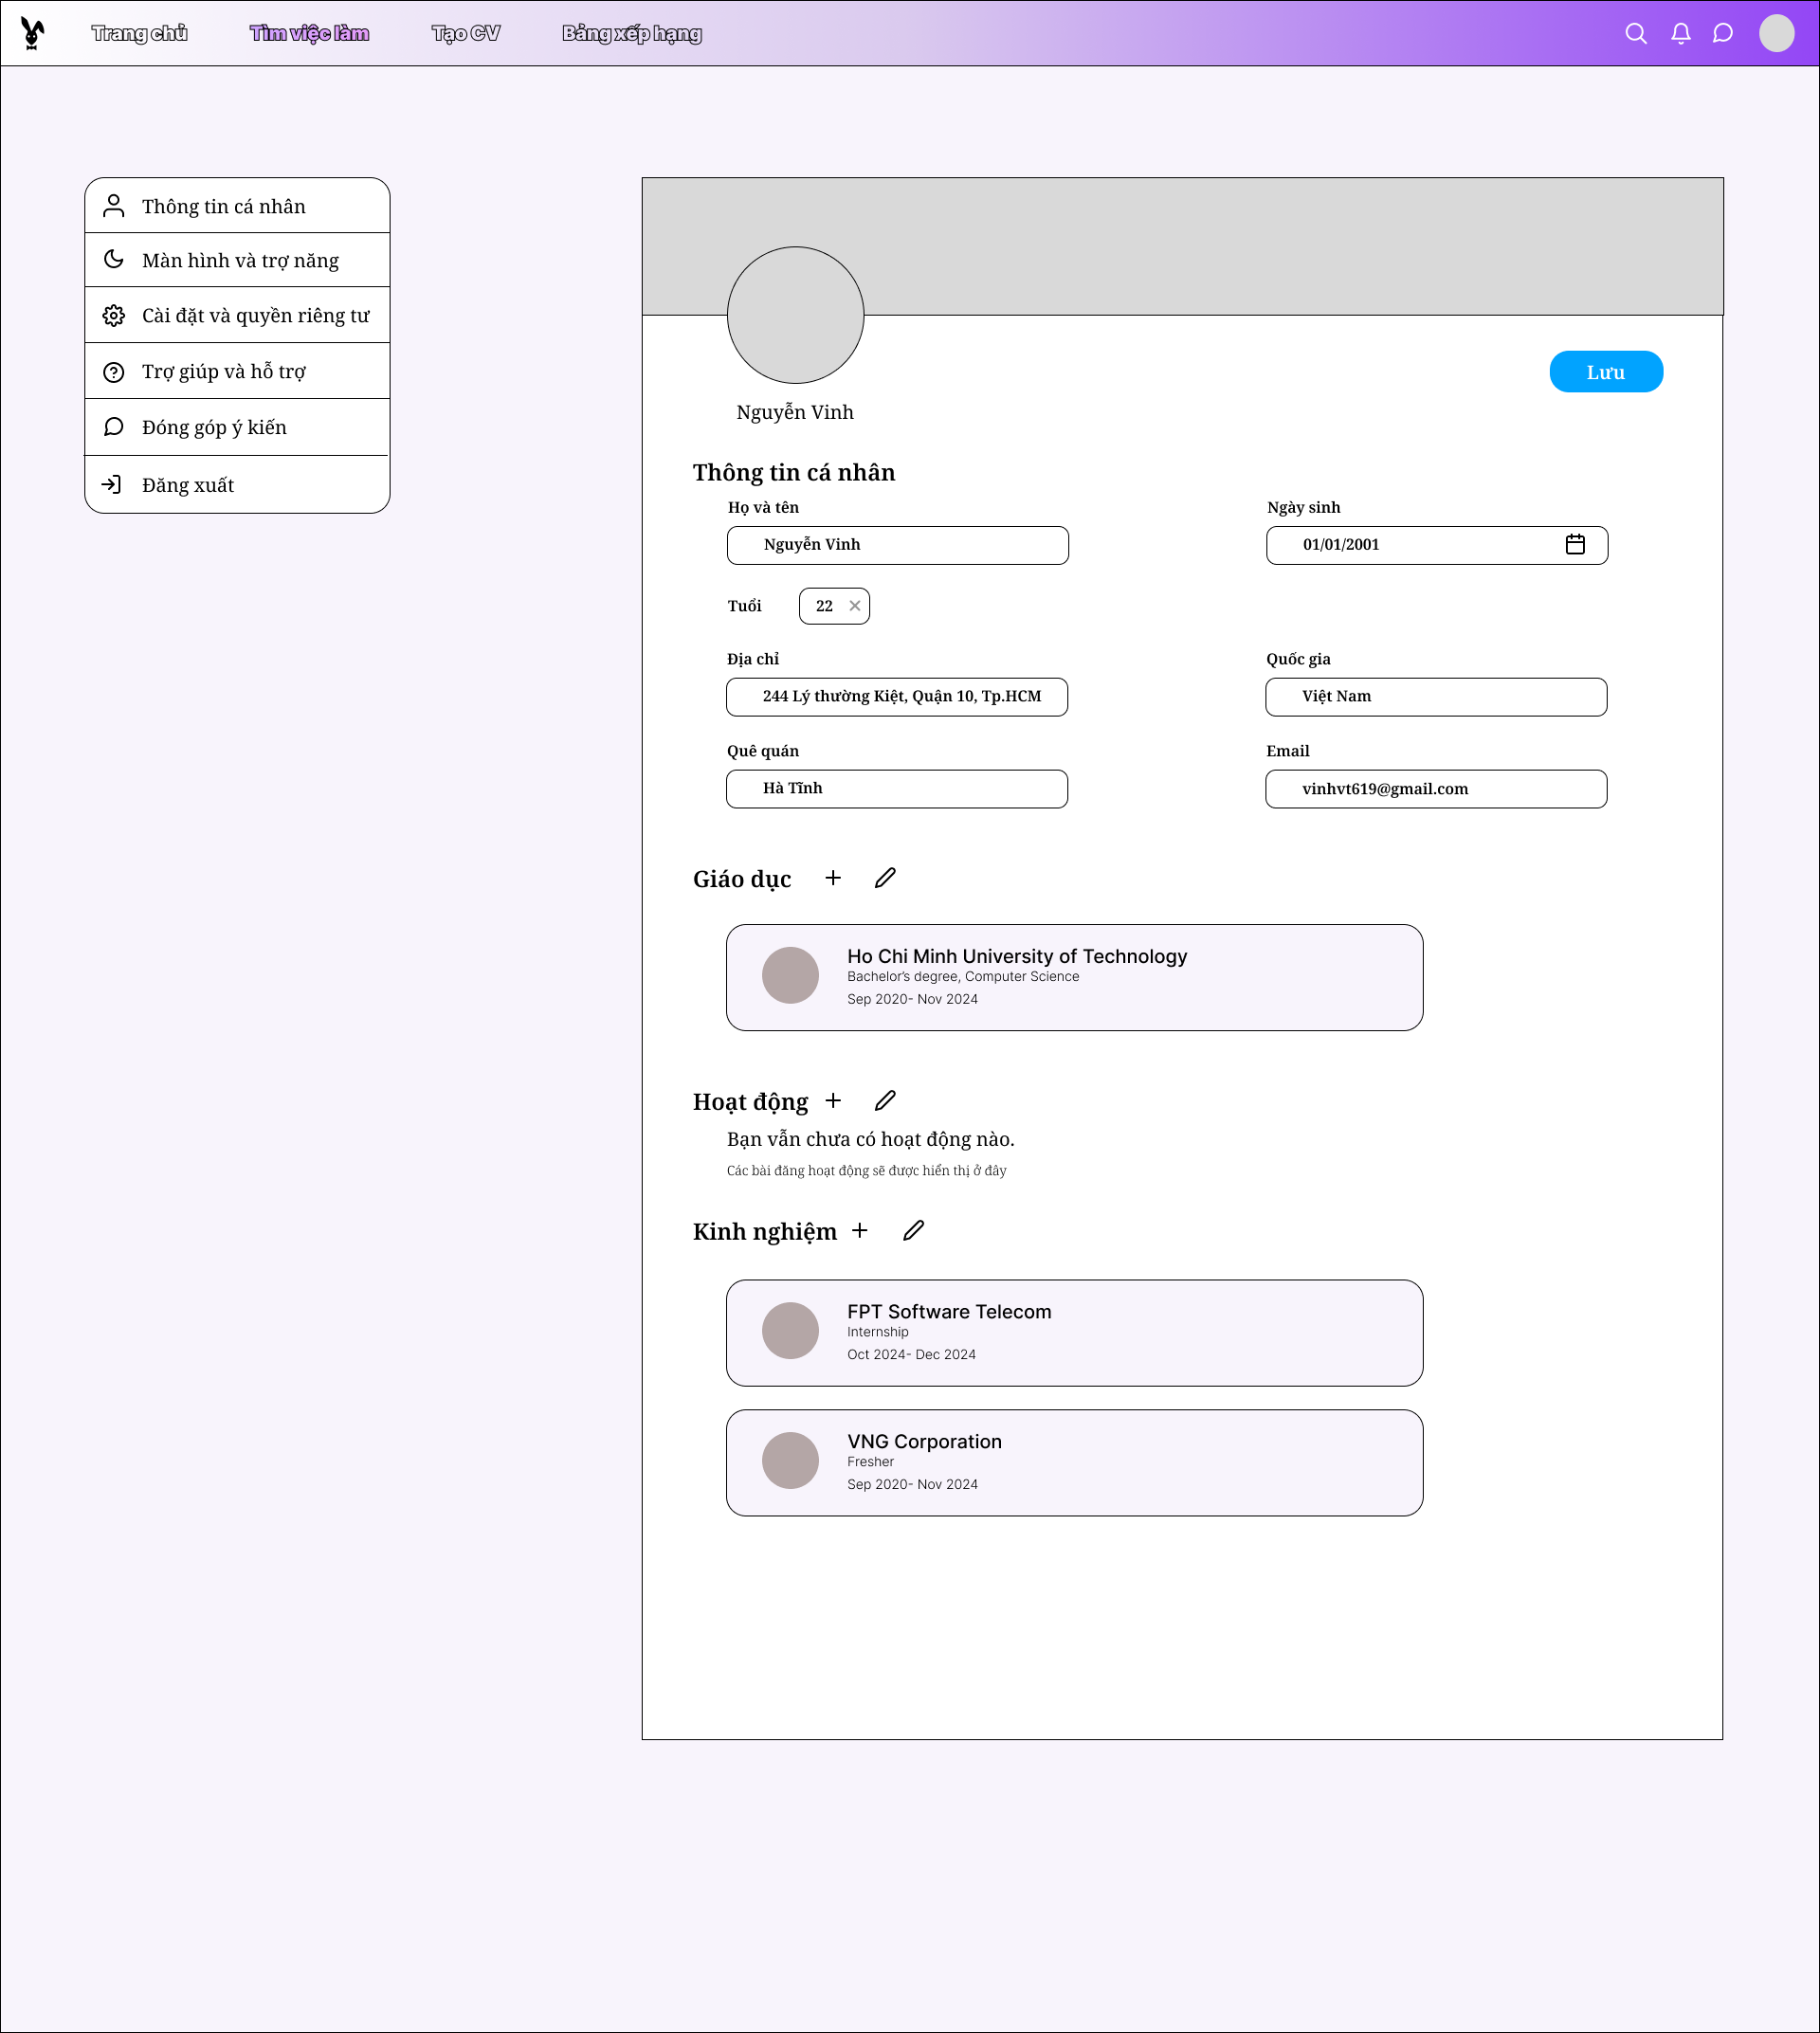
\includegraphics[scale=0.2]{img/ProfileManagement.png}
    \caption{Giao diện của Trang quản lý tài khoản}
\end{center}
\end{figure}

Là trang cài đặt gồm nhiều chức năng quản lý tài khoản. Ở đây, có nhiều mục cho người dùng có thể lựa chọn. Họ có thể lựa chọn để chỉnh sửa thông tin cá nhân của mình và thêm nhiều kỹ năng, kinh nghiệm của mình lên trang web.

Người dùng có thể lựa chọn màn hình tối đối với trang web phù hợp với thị hiếu của mình. Nếu người dùng có bất kỳ vấn đề và cần hỗ trợ hay muốn đóng góp ý kiến bản thân về trang web, họ có thể lựa chọn các mục "Trợ giúp và hỗ trợ" hay "Đóng góp ý kiến". Hệ thống sẽ chuyển hướng người dùng đến trang tương ứng và hướng dẫn người dùng cách thực hiện.